% !TeX program = lualatex
% !TeX root = ../../main.tex
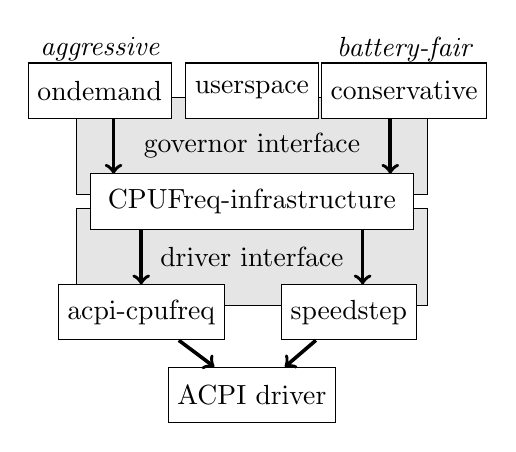
\begin{tikzpicture}[every node/.style={text centered}]
		\draw (0em, -2em)		node[draw, fill=gray!20%]
, text width=12em, minimum height=3.5em]
				{driver interface}

			(0em, 2em)		node[draw, fill=gray!20%]
, text width=12em, minimum height=3.5em]
				{governor interface}

			(0em, 0em)		node[draw, fill=white%]
, text width=11em, minimum height=2em] (cpuidle)
				{CPUFreq-infrastructure}



			(-5.5em, 4em)		node[draw, fill=white%]
, minimum height=2em] (ondemand)
				{ondemand}			
			(-5.5em, 5.5em)	node[font=\itshape] {aggressive}


			(5.5em, 4em)		node[draw, fill=white%]
, minimum height=2em] (conservative)
				{conservative}			
			(5.5em, 5.5em)	node[font=\itshape] {battery-fair}

			(0em, 4em)		node[draw, fill=white%]
, minimum height=2em] (userspace)
				{userspace}	



%			(-11em, 4em)	node {governors}
%			(-11em, -4em)	node {driver}
			
			(-4em, -4em)	node[draw%]
, minimum height=2em, fill=white] (acpifreq)
				{acpi-cpufreq}

(3.5em, -4em)	node[draw%]
, minimum height=2em, fill=white] (speedstep)
				{speedstep}



			(0em, -7em)	node[draw%]
, minimum height=2em, fill=white] (acpidriver)
				{ACPI driver}
			
;

	\draw[->, line width=1.3pt] (5em, 3em) -- (5em, 1em);%(menu) -- (cpuidle);
	\draw[->, line width=1.3pt] (-5em, 3em) -- (-5em, 1em);%(ladder) -- (cpuidle);

	\draw[<-, line width=1.3pt] (4em, -3em) -- (4em, -1em);%(haltidle) -- (cpuidle);
	\draw[<-, line width=1.3pt] (-4em, -3em) -- (-4em, -1em);%(acpiidle) -- (cpuidle);
	\draw[<-, line width=1.3pt] (acpidriver) -- (acpifreq);
	\draw[<-, line width=1.3pt] (acpidriver) -- (speedstep);
\end{tikzpicture}